To have a functioning beam, we need to introduce both the buffer gas as well as the target species gas from room temperature without over burdening the cooling stage, or plugging the fill lines. The buffer gas fill line is made of thin walled SS316, minimizing the thermal connection between the room temperature mounting and the cold experimental cell. It is thermally anchored to the 40K cooling stage and then brazed onto a plate that mounts to the experimental cell. To avoid local freezing of the buffer gas, the tubing must avoid cryopumping shield as contact.

More care must be taken for the design of the water fill line, as it cannot make contact with any mildly cooled metal surface for fear of local freezing. The mating of the fill line to the experimental cell must also prevent excessive heat loads onto the cell while still enclosing the back side to preserve beam flux. With the design help of David Patterson, we utilize a thick walled ~1/8" copper tube, with the tip bent at $90^\circ$, that enters from the bottom of the CBGB (figure \ref{fig: water fill bottom}), through the shields, into the back of the experimental cell. The fill line can be manipulated from the bottom of the chamber and the insertion depth into the cell can be adjusted before pump down. By slathering the o-ring at the bottom of the chamber with silicon vacuum grease, one may also adjust the tubing in situ, but the CBGB should be gated off from the rest of the experiment.

Leaving the back of the cell open eliminated conductive heat transfer between the fill line and the cell, but did not allow for a reliable beam. Ice readily formed on the nearby copper surfaces and slowly closed the back opening, decreasing the effective $A_{aperture}$ of the cell, thus changing the flow properties. The back was replaced with a 0.001" film of kapton with a cross cut into the middle for the fill line as seen in figure \ref{fig: kapton film}. The poor thermal conductivity of kapton (0.5 W/(m K)) ensures minimal conductive heat load to the cell, prevents ice from forming, while also closing the back of the cell. The beam may be run continuously with water entrained in the neon buffer gas for over 10 hours without any change in beam properties. Collisions with buffer gas particles within the cell transferring heat between the fill line and cell walls added $<0.05$W of heat load. Solving Fourier's Law in cylindrical coordinates (\ref{eq: cylindrical fourier}), we find that the heat load through the kapton is only 0.019 W.

\begin{equation}
	\dot{Q} = \frac{2 \pi k l (T_1 - T_2)}{\ln(r_2 - r_1)}
	\label{eq: cylindrical fourier}
\end{equation}

\begin{figure}[H]
	\centering
	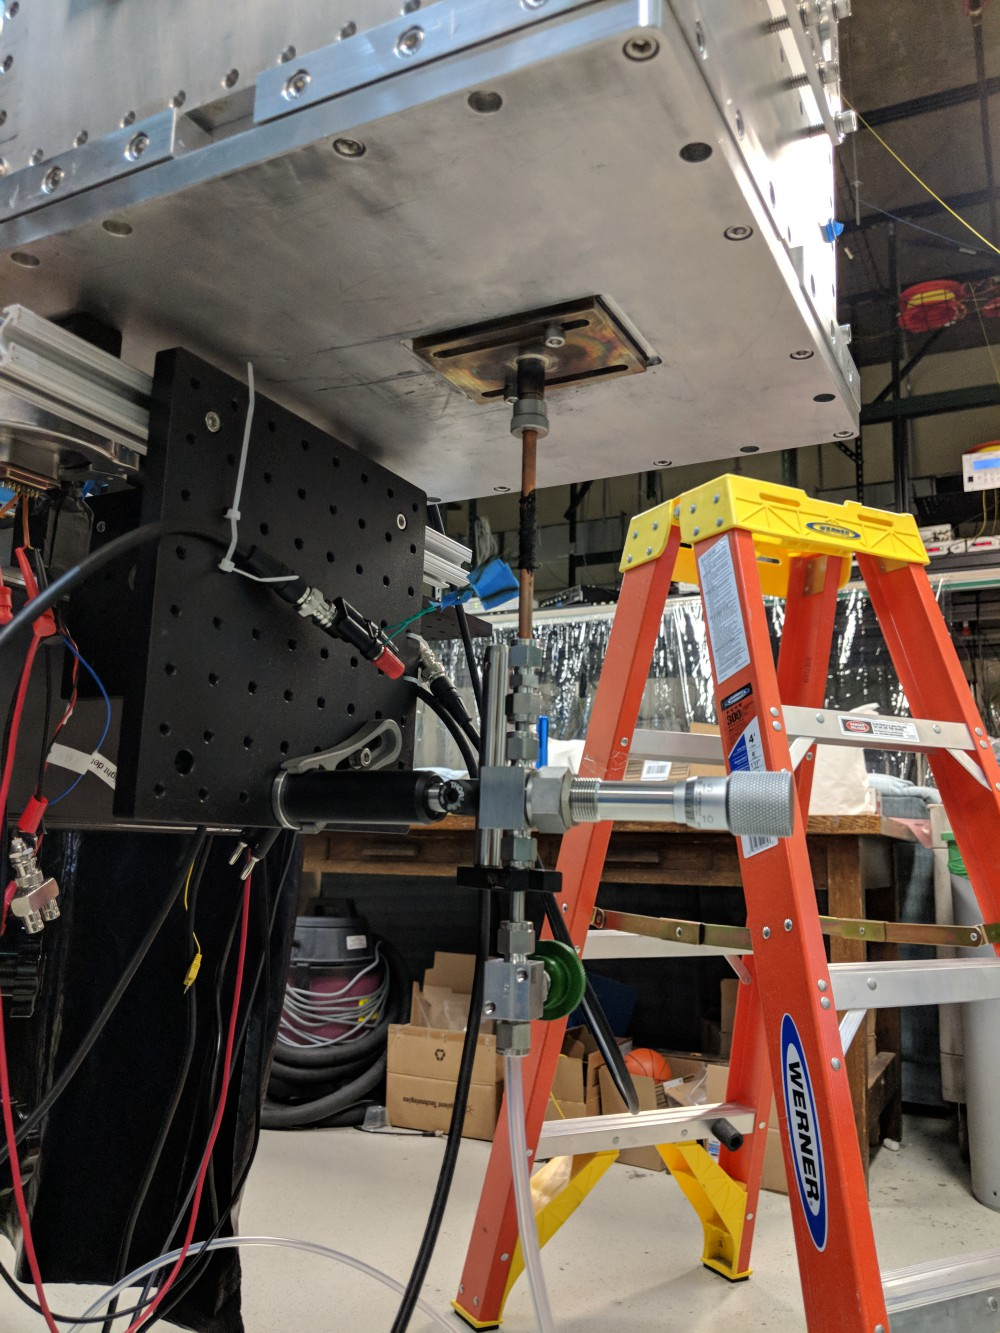
\includegraphics[width=.7\textwidth]{images/CBGB_water_fill_outside.jpg}
	\caption{The water fill line, sealed by an ultratorr fitting and heated by nichrome wire. A shut off valve and vernier valve are used to regulate the flow of water into the buffer gas cell.}
	\label{fig: water fill bottom}
\end{figure}

\begin{figure}[H]
	\centering
	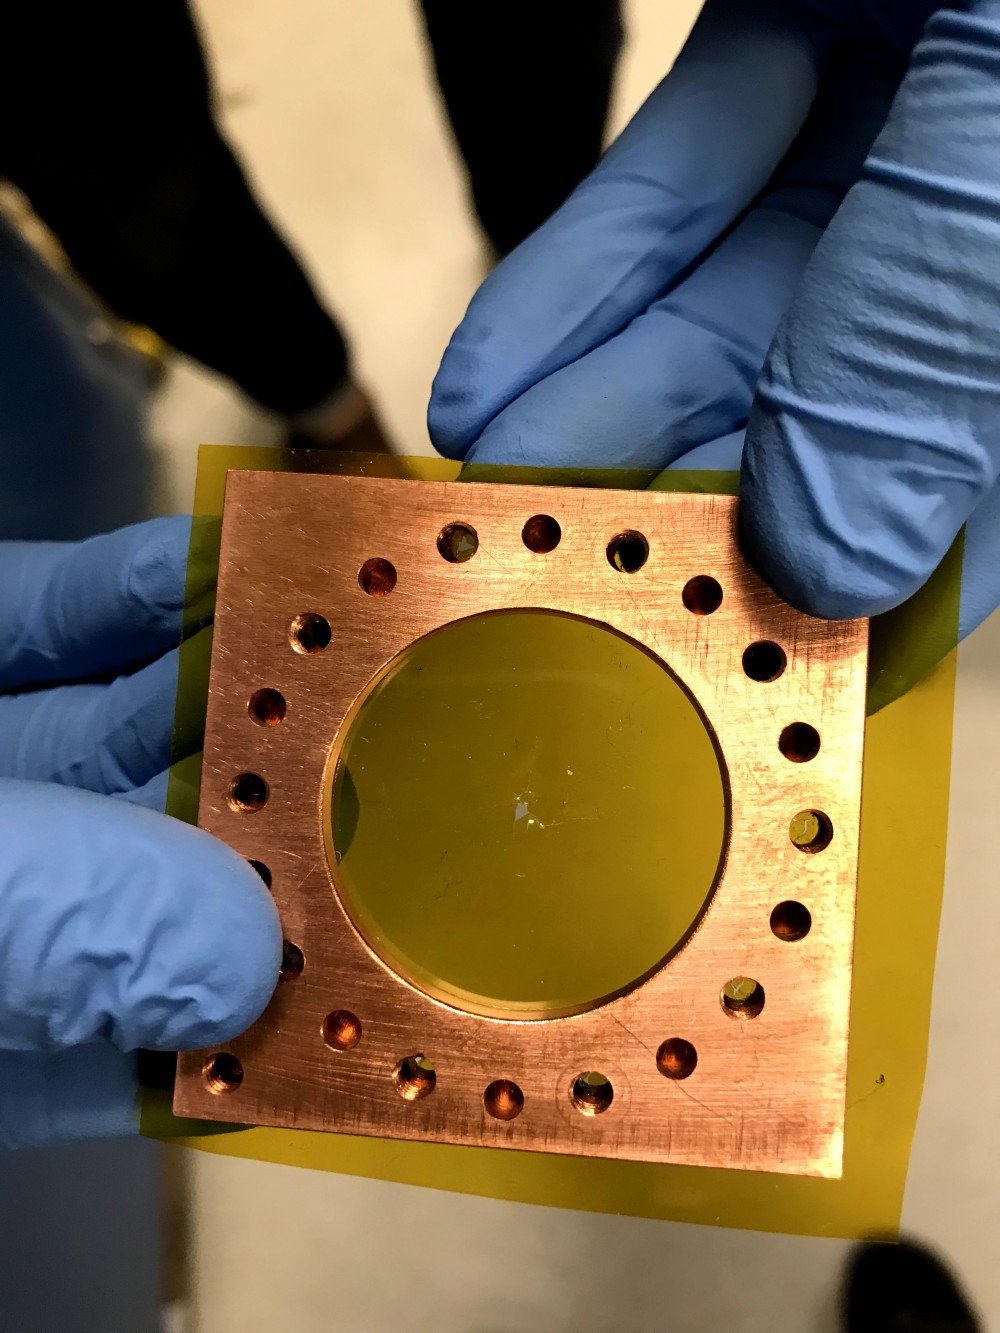
\includegraphics[width=.7\textwidth]{images/CBGB_kapton.jpg}
	\caption{A kapton film serves as the back wall of the buffer gas cell with a hole punctured for the insertion of the water fill line. The kapton surface seals the back of the cell for a stronger forward beam, while limiting the heat load from a room temperature fill line, and resisting ice formation allowing for continuous and consistent operation with water for over 10 hours.}
	\label{fig: kapton film}
\end{figure}